\documentclass[a4paper, 12pt]{article}
\usepackage[T2A]{fontenc}
\usepackage[utf8]{inputenc}
\usepackage[english,russian]{babel}
\usepackage{amsmath, amsfonts, amssymb, amsthm, mathtools, misccorr, indentfirst, multirow}
\usepackage{wrapfig}
\usepackage{graphicx}
\usepackage{subfig}
\usepackage{adjustbox}
\usepackage{pgfplots}

\usepackage{geometry}
\geometry{top=20mm}
\geometry{bottom=20mm}
\geometry{left=20mm}
\geometry{right=20mm}
\newcommand{\angstrom}{\textup{\AA}}


\title{Лабораторная работа 6.1\\Исследование резонансного поглощения $\gamma$-квантов (эффект Мессбауэра)}
\author{Нехаев Александр, гр. 654}
\date{\today}

\begin{document}
	\maketitle
	\pagenumbering{gobble}
	\newpage
	\pagenumbering{arabic}
	\tableofcontents
	\newpage
	\section{Введение}
	\paragraph{Цель работы:}
	С помощью метода доплеровского сдвига мессбауэровской линии поглощения исследуется резонансное поглощение $\gamma$-лучей, испускаемых ядрами олова $^{119}$Sn в соединении BaSnO$_3$ при комнатной температуре. Определяется положение максимума резонансного поглощения, его величина, а также экспериментальная ширина линии $\Gamma_{\text{экс}}$. Оценивается время жизни возбужденного состояния ядра $^{119}$Sn.
	\paragraph{В работе используются:}
	(См рис. \ref{fig1})
	Э – эксцентрик,
	С – сцинтилляционный кристалл NaI(Tl), У – усилитель, АА – одноканальный амплитудный анализатор, ЭВМ – ПК, Г – генератор питания двигателя, РД-09 – двигатель с редуктором, ВСВ – высоковольтный стабилизированный выпрямитель.\par
	\begin{figure}[h]
		\centering
		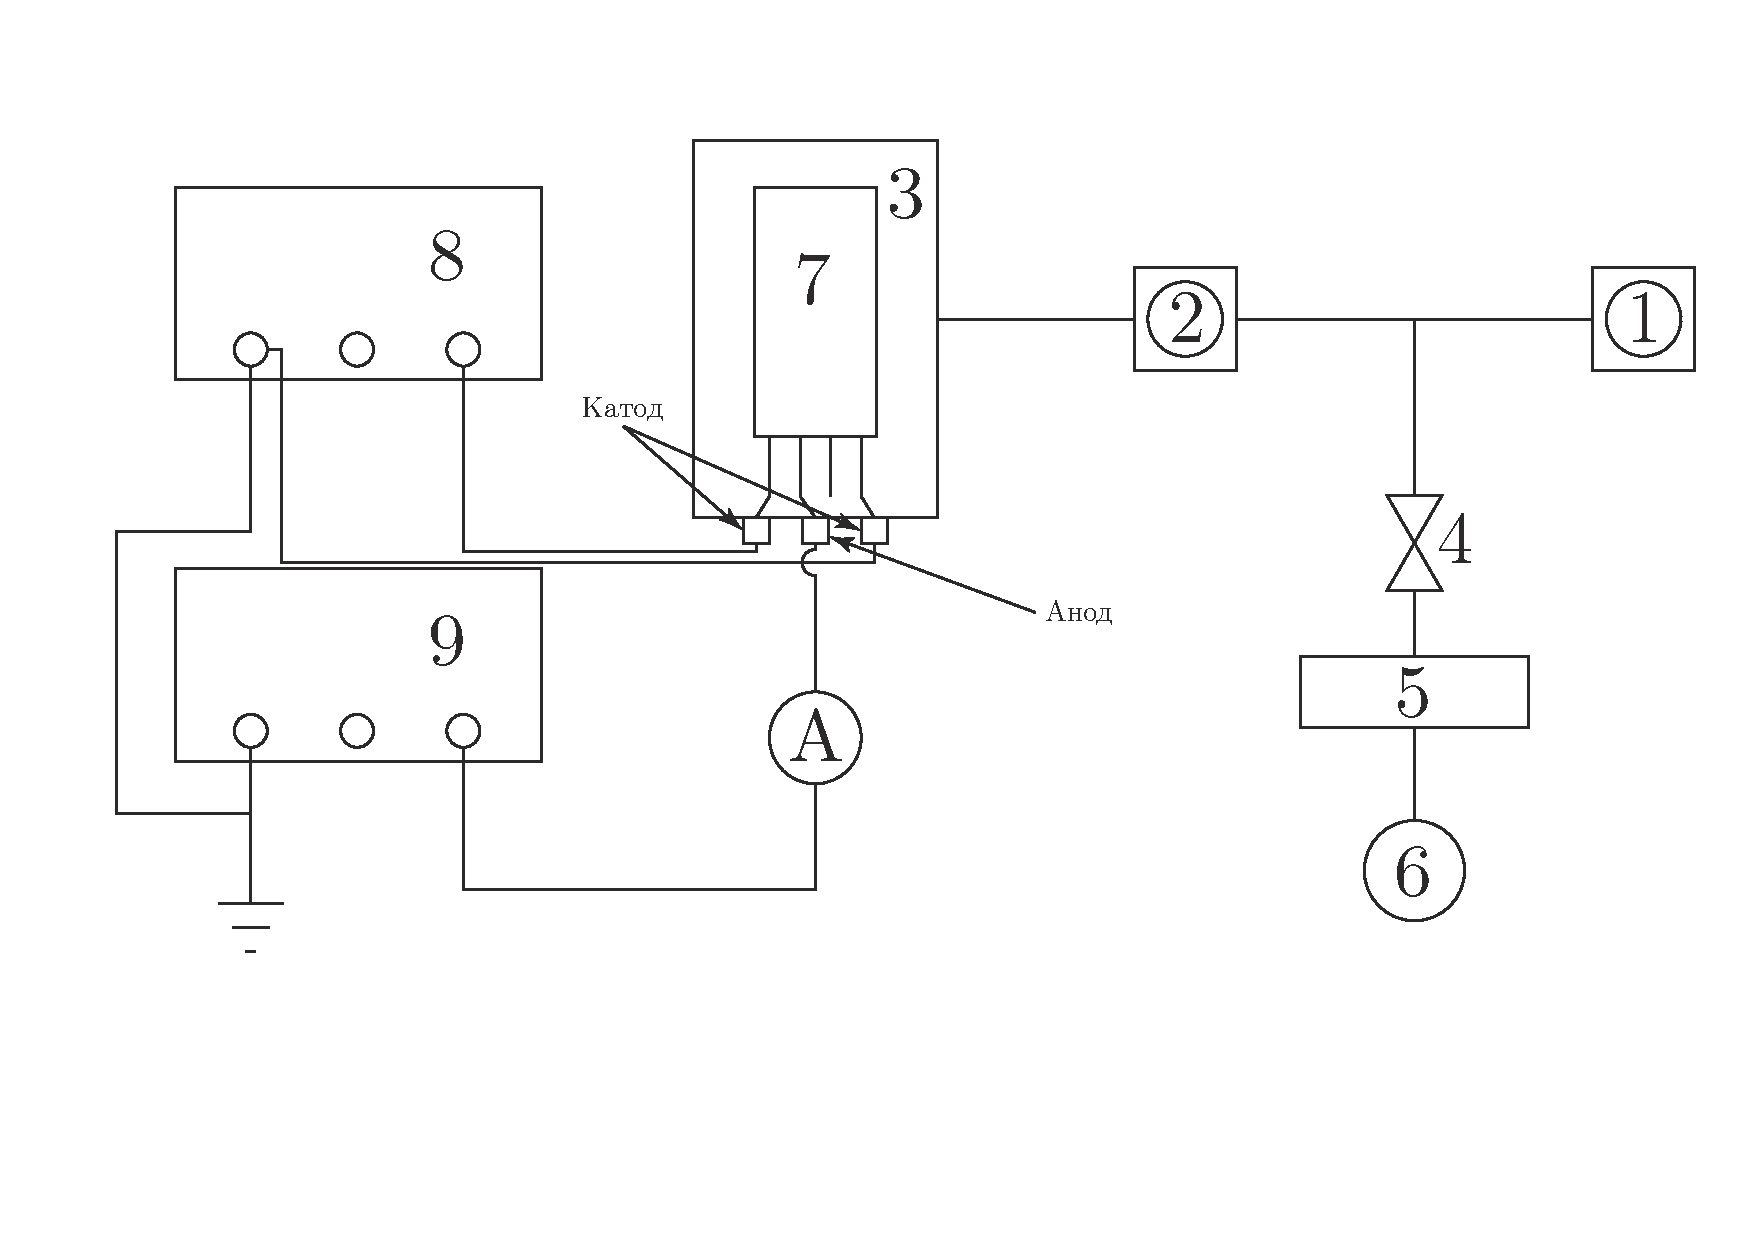
\includegraphics[scale=0.2]{scheme.png}
		\caption{Схема экспериментальной установки}
		\label{fig1}
	\end{figure}
	\paragraph{Теоретические основы}
	Нуклоны в атомном ядре, как и электроны в атоме, могут находиться в различных дискретных энергетических состояниях, или, как говорят, на различных энергетических уровнях. Самый низкий из уровней называется основным, остальные носят название возбужденных. Ядра, находящиеся в возбужденных состояниях, могут переходить на более низкие энергетические уровни, в том числе и на основной уровень. Такие переходы происходят самопроизвольно. Освобождающаяся энергия уносится фотоном. Так  возникает $\gamma$-излучение.\par
	\begin{wrapfigure}{1}{5cm}
		\includegraphics[scale=0.2]{energy.png}
		\caption{Энергетическое распределение, характеризующее возбужденное состояние ядра (а), и сдвиг линий испускания и поглощения из-за отдачи при свободных ядрах(б).}
		\label{figT2}
	\end{wrapfigure}
	В отличие от основного уровня, все возбужденные уровни ядра имеют конечную ширину. Отложим по оси абсцисс энергию ядра, а по оси ординат – вероятность найти ядро в состоянии с данной энергией (рис. \ref{figT2}а). Ширина кривой, измеренная на половине высоты, называется естественной шириной линии $\Gamma$. Она связана со средним временем жизни $\tau$ возбужденного состояния ядра соотношением неопределенностей
	\begin{equation}
		\Gamma\tau\simeq\hbar
	\end{equation}
	где $\hbar$ — постоянное Планка. Неопределенность в энергии возбужденных уровней приводит к появлению ширины у линий $\gamma$-излучения.\par
	Ядра атомов могут не только испускать, но и поглощать фотоны. Если попадающий в атомное ядро фотон имеет энергию, равную разности энергий между основным и каким-либо возбужденным состояниями, то ядро может поглотить фотон и перейти в соответствующее возбужденное состояние. Этот процесс возможен лишь для $\gamma$-лучей определенных энергий и носит, таким образом, резонансный характер.\par
	Энергия $E_\gamma$, уносимая $\gamma$-квантом, оказывается меньше энергии $E_0$ перехода между уровнями. Небольшая, но вполне заметная доля энергии уносится ядром, которое вследствие отдачи начинает двигаться в сторону, противоположную направлению вылета $\gamma$-кванта.\par
	Ядро, которое испускает $\gamma$-квант, приобретает импульс отдачи, равный по абсолютной величине импульсу $\gamma$-кванта. Если ядро свободно и первоначально покоится, то энергия отдачи $R$ равна
	\begin{equation}
		R=\frac{p^2}{M_{\text{я}}}=\frac{E_{\gamma}^2}{2M_{\text{я}}c^2}.
		\label{eq:2}
	\end{equation}
	\par
	Рассмотрим в качестве примера ядро олова $^{119}$Sn, у которого расстояние между основным и первым возбужденным уровням равно $E_0=23.8$ кэВ. Энергия отдачи в этом случае составляет\footnote{Величины $E_0$, $E_\gamma$ и $R$ связаны законом сохранения энергии: $E_0=E_\gamma+R$. Поскольку $R\ll E_\gamma$, в формуле (\ref{eq:2}) $E_\gamma$ можно заменить на энергию возбужденного состояния $E_0$.}
	\begin{equation*}
		R=\frac{E_\gamma^2}{2M_{\text{я}}c^2}\simeq\frac{E_0^2}{2M_\text{я}c^2}=2.5\cdot10^{-3}\text{ эВ}.
	\end{equation*}
	\par
	Энергия, которая расходуется на отдачу ядра, поглощающего $\gamma$-квант, оказывается точно такой же. Эта картина иллюстрирует рис.\ref{figT2}б: линия испускания смещена на величину $R$ влево, а линия поглощения – на столько же вправо от $E_0$.\par
	Обсуждая влияние, которое оказывает сдвиг $R$ на резонансное поглощение $\gamma$-лучей, следует иметь в виду, что величина $R$ сама по себе не представляет существенного интереса. Важно соотношение между $R$ и шириной $\Gamma$ соответствующей резонансной линии. Резонансное поглощение возможно только в том случае, если спектры испускания и поглощения перекрываются, т.е. при условии
	\begin{equation}
		2R\leqslant\Gamma.
	\end{equation}
	\par
	Это условие почти никогда не выполняется для $\gamma$-переходов в свободных ядрах. Так, для рассмотренного ядра $^{119}$Sn естественная ширина линии $\Gamma\simeq3\cdot10^{-8}$ эВ, т.е. на много порядков величины меньше $R$\footnote{Заметим, что при оптических переходах в атомах соотношение между $R$ и $\Gamma$ существенно меняется. В этом случае энергии переходов оказываются на 4 порядка и, следовательно, $R$ на 8 порядков величины меньше, чем при $\gamma$-излучении, а ширины уровней оказываются, грубо говоря, того же порядка. В этом случае поглощение легко наблюдается.}. В принципе, можно компенсировать энергетический сдвиг $2R$ с помощью эффекта Доплера. Для этого изучающие и поглощающие ядра должны двигаться друго относительно друга со скоростью $V$, равной
	\begin{equation}
		V=c\cdot2R/E_\gamma.
	\end{equation}
	\par
	Для ядер $^{119}$Sn нужна скорость $V\simeq60$ м/с.\par
	В реальных условиях ширина линии испускания (и поглощения) складывается из собственной ширины линии и её доплеровской ширины. Из этих двух ширин основную роль играет именно доплеровская ширина уровней, связанная с тепловым движением атомов.
	\section{Ход работы}
	\subsection{Измерение спектра источника}
	\begin{enumerate}
		\item Включим приборы и после прогрева установим напряжение на ФЭУ. Включим компьютер.
		\item Изменяя нижний порог окна сцинтилляционного спектрометра шириной $0.5$ В, измерим спектр источника:
		\begin{table}[h]
			\centering
			\begin{tabular}{|c|c|c|}
				\hline
				Номер & Нижний порог & Интенсивность\\
				\hline
				1 & 0.0 & 145862.6\\
				2 & 0.5 & 350.0\\
				3 & 1.0 & 771.2\\
				4 & 1.5 & 179.6\\
				5 & 2.0 & 26.2\\
				6 & 2.5 & 33.0\\
				7 & 3.0 & 70.8\\
				8 & 3.5 & 109.8\\
				9 & 4.0 & 151.0\\
				10 & 4.5 & 178.6\\
				11 & 5.0 & 196.8\\
				12 & 5.5 & 183.8\\
				13 & 6.0 & 143.0\\
				14 & 6.5 & 83.6\\
				15 & 7.0 & 47.8\\
				16 & 7.5 & 23.2\\
				17 & 8.0 & 10.8\\
				18 & 8.5 & 5.8\\
				19 & 9.0 & 6.0\\
				20 & 9.5 & 4.6\\
				\hline
			\end{tabular}
			\caption{Значения спектра источника}
		\end{table}
		\item Построим график $I=f\left(U_1\right)$ (рис. \ref{graph1}).
		\begin{figure}[h]
			\begin{tikzpicture}
				\begin{axis}[
					title={$I=f\left(U_1\right)$},
					xlabel={$U_1$, В},
					ylabel={$I$, c$^{-1}$},
					xmin=0.0,
					xmax=10.0,
					ymin=0.0,
					ymax=210.0,
					ymajorgrids=true,
    				xmajorgrids=true,
    				grid style=dashed,
    				width=\textwidth,
				]
				\addplot+[
					color=black,
    				mark=square,
    				only marks,
					error bars/.cd,
					y dir=both, y explicit,
					x dir=both, x explicit
				]
				coordinates{
					(2.0, 26.2)+-(0.1, 1.048)
					(2.5, 33.0)+-(0.1, 1.32)
					(3.0, 70.8)+-(0.1, 2.832)
					(3.5, 109.8)+-(0.1, 4.392)
					(4.0, 151.0)+-(0.1, 6.04)
					(4.5, 178.6)+-(0.1, 7.144)
					(5.0, 196.8)+-(0.1, 7.872)
					(5.5, 183.8)+-(0.1, 7.352)
					(6.0, 143.0)+-(0.1, 5.72)
					(6.5, 83.6)+-(0.1, 3.344)
					(7.0, 47.8)+-(0.1, 1.912)
					(7.5, 23.2)+-(0.1, 0.928)
					(8.0, 10.8)+-(0.1, 0.432)
					(8.5, 5.8)+-(0.1, 0.232)
					(9.0, 6.0)+-(0.1, 0.24)
					(9.5, 4.6)+-(0.1, 0.184)
				};
				\addplot[
					domain=0:10,
					samples=200,
					color=black
				]
				{192.906*exp((-0.289343)*(x-4.87281)^2)};
				\end{axis}
			\end{tikzpicture}
			\caption{Спектр источника}
			\label{graph1}
		\end{figure}
		\par
		Аппроксимируем график по Гауссовскому распределению вида
		\begin{equation*}
			y=\frac{A\cdot e^{-\frac{(x-x_0)^2}{2\sigma^2}}}{\sqrt{2\pi}\sigma}
		\end{equation*}
		и получаем коэффициенты
		\begin{equation*}
			A=(635.64\pm18.84), x_0=(4.87\pm0.04), \sigma=(1.314\pm0.033)
		\end{equation*}
		упрощая, получаем уравнение
		\begin{equation*}
			y=(192.9\pm7.5) e^{-(0.29\pm0.03) (x-(4.87\pm0.04))^2}
		\end{equation*}
		Из графика, с учетом аппроксимации находим, что энергия 23.8 эВ соответствует значению $U_1=4.87$ В.
		\subsection{Измерение резонансного поглощения}
		\item Установим окно сцинтилляционного спектрометра, соответствующее ширине линии спектра излучения $3.5-7$ В, и проведем измерения резонансного поглощения:
		\begin{enumerate}
			\item Поглощение на Sn(100$\mu$)
			\item Поглощение на Sn(200$\mu$)
			\item Поглощение на SnO$_2$
			\begin{table}[h]
				\begin{minipage}{0.49\textwidth}
				\begin{tabular}{|c|c|c|c|c|}
					\hline
					№ & $v_-$ & $I_-$ & $v_+$ & $I_+$\\
					\hline
					1 & 1.44 & 871.7 & 1.52 & 853.3 \\
 					2 & 1.52 & 852.1 & 1.61 & 850.1 \\
				 	3 & 1.48 & 858.4 & 1.59 & 843.1 \\
 					4 & 1.37 & 852.4 & 1.51 & 853.6 \\
 					5 & 1.21 & 834.4 & 1.35 & 842.6 \\
 					6 & 4.44 & 856.6 & 4.71 & 848.4 \\
 					7 & 3.71 & 845.9 & 3.92 & 846.7 \\
 					8 & 3.08 & 857.9 & 3.27 & 840.0 \\
 					9 & 2.48 & 847.0 & 2.64 & 750.8 \\
 					10 & 2.12 & 841.9 & 1.67 & 838.1 \\
 					11 & 1.57 & 858.0 & 1.64 & 837.1 \\
	 				12 & 1.55 & 841.3 & 1.16 & 841.4 \\
 					13 & 1.06 & 857.6 & 2.79 & 764.0 \\
 					14 & 2.62 & 869.2 & 3.0 & 793.3 \\
 					15 & 2.83 & 869.1 & 3.16 & 812.6 \\
 					16 & 2.99 & 852.9 & 3.49 & 828.7 \\
 					17 & 2.16 & 850.5 & 3.12 & 815.8 \\
 					18 & 1.85 & 856.1 & 2.82 & 778.5 \\
 					19 & 2.34 & 854.7 & 2.32 & 762.0 \\
 					20 & 2.11 & 858.0 & 1.99 & 812.8 \\
	 				21 & 1.93 & 838.0 & 2.48 & 755.3 \\
 					22 & 2.25 & 845.6 & 2.22 & 792.8 \\
 					23 & 3.28 & 849.8 & 2.04 & 799.9 \\
	 				24 & 2.94 & 847.7 & 2.41 & 764.4 \\
 					25 & 2.66 & 855.3 & 2.24 & 791.3 \\
					\hline
				\end{tabular}
				\caption{Поглощение на Sn($100\mu$)}
				\end{minipage}
				\hfil
				\begin{minipage}{0.55\textwidth}
				\begin{tikzpicture}
					\begin{axis}[
						title={Sn($100\mu$)},
						xlabel={$v$, мм/с},
						ylabel={$I$, c$^{-1}$},
						xmin=-5,
						xmax=5,
						ymin=750.0,
						ymax=900.0,
						ymajorgrids=true,
    					xmajorgrids=true,
    					grid style=dashed,
    					width=\textwidth,
    					height=14cm
					]
					\addplot+[
						color=black,
    					mark=square,
    					only marks,
						error bars/.cd,
						y dir=both, y explicit,
						x dir=both, x explicit
					]
					coordinates{
					(-1.44, 871.7)+-(0,0)
					(-1.52, 852.1)+-(0,0)
					(-1.48, 858.4)+-(0,0)
					(-1.37, 852.4)+-(0,0)
					(-1.21, 834.4)+-(0,0)
					(-4.44, 856.6)+-(0,0)
					(-3.71, 845.9)+-(0,0)
					(-3.08, 857.9)+-(0,0)
					(-2.48, 847.0)+-(0,0)
					(-2.12, 841.9)+-(0,0)
					(-1.57, 858.0)+-(0,0)
					(-1.55, 841.3)+-(0,0)
					(-1.06, 857.6)+-(0,0)
					(-2.62, 869.2)+-(0,0)
					(-2.83, 869.1)+-(0,0)
					(-2.99, 852.9)+-(0,0)
					(-2.16, 850.5)+-(0,0)
					(-1.85, 856.1)+-(0,0)
					(-2.34, 854.7)+-(0,0)
					(-2.11, 858.0)+-(0,0)
					(-1.93, 838.0)+-(0,0)
					(-2.25, 845.6)+-(0,0)
					(-3.28, 849.8)+-(0,0)
					(-2.94, 847.7)+-(0,0)
					(-2.66, 855.3)+-(0,0)
					(1.52, 853.3)+-(0,0)
					(1.61, 850.1)+-(0,0)
					(1.59, 843.1)+-(0,0)
					(1.51, 853.6)+-(0,0)
					(1.35, 842.6)+-(0,0)
					(4.71, 848.4)+-(0,0)
					(3.92, 846.7)+-(0,0)
					(3.27, 840.0)+-(0,0)
					(2.64, 750.8)+-(0,0)
					(1.67, 838.1)+-(0,0)
					(1.64, 837.1)+-(0,0)
					(1.16, 841.4)+-(0,0)
					(2.79, 764.0)+-(0,0)
					(3.0, 793.3)+-(0,0)
					(3.16, 812.6)+-(0,0)
					(3.49, 828.7)+-(0,0)
					(3.12, 815.8)+-(0,0)
					(2.82, 778.5)+-(0,0)
					(2.32, 762.0)+-(0,0)
					(1.99, 812.8)+-(0,0)
					(2.48, 755.3)+-(0,0)
					(2.22, 792.8)+-(0,0)
					(2.04, 799.9)+-(0,0)
					(2.41, 764.4)+-(0,0)
					(2.24, 791.3)+-(0,0)
					};
					\end{axis}
				\end{tikzpicture}
				\end{minipage}
			\end{table}
		\end{enumerate}
	\end{enumerate}
\end{document}